%------------------------------------------------------------------------------------------------------------------------------------------------------------------------
\chapter{RTF Exploration and Feasibility Study}\label{init_eval}
%------------------------------------------------------------------------------------------------------------------------------------------------------------------------

We perform 2 studies to test the potential of PACORA for resource allocation.

\subsection{RTF Exploration and System Potential using an FPGA-based System Simulator}
~\cite{bird,tess_resource}



\subsubsection*{Experimental Setup}

We performed some of our own resource allocation experiments to
confirm that runtime hardware measurements can help improve OS
scheduling decisions.  Using an FPGA-based multiprocessor emulator RAMP Gold~\cite{rampgold09, rampgold10, fame10} and
a simple research operating system ROS~\cite{ros, tess,tess_resource}, we ran experiments with the Parsec
2.0 Benchmark Suite~\cite{parsec} and some handcrafted
microbenchmarks on a 64-core target machine. The OS uses page coloring
to allocate sections of the cache to an application, and the simulator
implements a simple form of bandwidth partitioning by limiting the
number of requests that can be sent to memory over a time
interval. Our system executes each of the applications several times,
each time varying the number of cores, and cache and bandwidth
allocations.  We collect application runtime performance data using
performance measurement hardware to create models of the performance
for that application given a particular resource allocation.  We
created a quadratic model and linear model with multivariate
regression techniques, a GPRS model, and a KCCA model using 20\% of the possible allocations.  Using
these models, our scheduler decides how best to run a mix of two
applications by trying to optimize a given objective function.  For
these results, we chose a simple proxy for total energy consumed, the
total number of cycles run (the sum of the cycles on each core) +
10$\times$ the total number of off-chip accesses, as our example
objective function.

Our experimental platform for this case study consists of five Xilinx
XUP FPGA boards. Each board is programmed to simulate one instance of
our target architecture.  Table~\ref{table:target} lists the target
machine parameters. We run six applications from the PARSEC benchmark
suite \cite{parsec}, as well as two synthetic microbenchmarks.
Table~\ref{table:benchmarks} summarizes the benchmarks. The
performance models are built based on applications running alone on a
partition of the machine but are tested against data collected from
multiprogrammed scheduling scenarios.  We simulated all possible
allocations for each benchmark running alone, and then all possible
schedules of allocations for 3 pairs of benchmarks running
simultaneously, for a combined total of 68.5 trillion target
core-cycles.  (A core-cycle is 1 clock cycle of execution on 1 core;
simulating a 64-core CMP for 1,000,000 cycles would be 64,000,000
core-cycles.)

 The Research Operating System (ROS) is a prototype operating system
 build to investigate OS design principles in the manycore era
 \cite{tess, tess_resource, tess_dac}.  We ported ROS to boot on Midas FAME, and
 modified its functionality to support our scheduling framework
 (including paging management and threading libraries).


Our spatial scheduling framework is implemented within a prototype
research operating system (ROS) that runs on the target machine
simulated by Midas FAME~\cite{ros}.


\begin{table*}[ct]
 \begin{center}
\footnotesize
\begin{tabular}{|c|l|}
\hline
 Attribute  & Setting \\ \hline \hline
 CPUs & 64 single-issue in-order cores @ \wunits{1}{GHz} \\ \hline
 L1 Instruction Cache & Private, \wunits{32}{KB}, 4-way set-associative, 128-byte lines \\ \hline
 L1 Data Cache & Private, \wunits{32}{KB}, 4-way set-associative, 128-byte lines \\ \hline
 L2 Unified Cache & Shared, \wunits{8}{MB}, 16-way set-associative, 128-byte lines, inclusive, 4 banks, \wunits{10}{ns} latency \\ \hline
 Off-Chip DRAM & \wunits{2}{GB}, 4$\times$\wunits{3.2}{GB/sec} channels,
 \wunits{70}{ns} latency \\ \hline
 \end{tabular}
\caption{Target machine parameters simulated by RAMP Gold.}
\label{table:target}
 \end{center}
\end{table*}

\begin{table*}[ct]
 \begin{center}
\footnotesize
\begin{tabular}{|l|l|l|r|l|}
\hline
 Name  & Type & Parallelism & Working Set & Bandwidth Demand\\ \hline \hline
Blackscholes & financial PDE solver & coarse data parallel & \wunits{2.0}{MB} & minimal \\ \hline
Bodytrack & vision & medium data parallel & \wunits{8.0}{MB} & grows with cores\\ \hline
Fluidanimate & animation & fine data parallel & \wunits{64.0}{MB} & grows with cores\\ \hline
Streamcluster & data mining & medium data parallel & \wunits{16.0}{MB} & high \\ \hline
Swaptions & financial simulation & coarse data parallel & \wunits{0.5}{MB} & grows with cores \\ \hline
x264 & media encoder & pipeline & \wunits{16.0}{MB} & grows with cores \\ \hline \hline
Tiny & synthetic &  one thread does all work & \wunits{1}{KB} & minimal \\ \hline
Greedy & synthetic & data parallel & \wunits{16.0}{MB} & high \\ \hline
\end{tabular}
\caption{Benchmark description. PARSEC benchmarks use \texttt{ simlarge} input set sizes, except for x264 and fluidanimate, which use \texttt{ simmedium} due to limited physical memory capacity.  PARSEC characterizations are from \cite{parsec}.}
\label{table:benchmarks}
 \end{center}
\end{table*}


\paragraph*{Partitioning Mechanisms}
Our allocation framework includes the following resources: the cores
and their private caches, the shared last-level cache, and shared
memory bandwidth.  For each resource, we provide a mechanism to
prevent applications from exceeding their allocated share. The OS
assigns cores and their associated private resources to a specific
application. For the shared last-level cache, we modify the OS
page-coloring algorithm so that applications are never given a page
from a different application's color allocation.

To partition off-chip memory bandwidth, we use Globally-Synchronized
Frames (GSF)\cite{gsf}. GSF provides strict Quality-of-Service
guarantees for minimum bandwidth and the maximum delay of a
point-to-point network---in our case the memory network---by
controlling the number of packets that each core can inject per frame.
We use a modified version of the original GSF design, which tracks
allocations per application instead of per core, does not reclaim
frames early, and does not allow applications use the excess
bandwidth.  These changes make GSF more suited to our study since we
want to strictly bound the maximum bandwidth per application.
Implementing GSF required some modifications to the target machine's
memory controller in RAMP Gold to synchronize the frames and track
application packet injections.  Due to the functional/timing split in
RAMP Gold, this modification was no more difficult than modifying a
software simulator would have been.

\paragraph{RTF Construction}

 We use a design of experiments (DoE) technique known as the Audze-Eglais
Uniform Latin Hypercube design of experiments \cite{bates-aes03} to
select the points included in the sample set.  %Audze-Eglais selects
%sample points which are as evenly distributed as possible through the
%space of possible allocations.

To explore the relationship between model accuracy and model type
for our problem space, we evaluate linear additive models, quadratic
response surface models, and non-linear models based on Kernel Canonical Correlation Analysis (KCCA) \cite{kcca} and GPRS.

The simplest models we consider are linear additive models, which
contain one term for each variable (i.e. an allocation type) and one
coefficient associated which each term.  Linear additive models
ignore any possible interaction between the variables, an invalid
assumption in our scheduling scenario.  For this reason, we also
include more complex multivariate regression models, commonly termed
`response surface models', which include terms for variable
interaction and polynomial terms of degree 2 or more.  We also employ
Kernel Canonical Correlation Analysis (KCCA) \cite{kcca} as a
representative example of even more complex nonlinear modeling
techniques. KCCA automatically detects correlations among the
variables and outputs included in the model, and uses this analysis
to make predictions.


\paragraph{Resource Allocation Decisions}

The scheduler uses the models for each application to decide how best
to divide resources up between a mix of applications all running
concurrently.  Our initial prototype scheduler optimizes the
reassignment of spatial resource allocations without regard to the
current allocations and the resulting reallocation overhead.  Even
this simplified problem is combinatorial (and in fact is
NP-hard). The algorithm works by maximizing an objective function,
which serves to convert model outputs into a measure of overall
decision fitness.  The form of the objective function influences the
type of algorithm we can use to maximize fitness. We use Matlab's
\cite{matlab} implementation of the medium-scale active-set
algorithm, which is a sequential quadratic programming based solver
and so depends on the convexity of the function to guarantee
optimality.

Only some of our objective functions are convex, and the optimization
algorithm may choose local minima for ones which are not.  As a
result, even with perfect models the scheduler could pick non-optimal
solutions.  For this reason, it is important to experiment with
different model types, sample sizes, objective functions, and
maximization algorithms to find the right balance between system
complexity and accuracy of scheduling decisions.




\subsubsection*{Case Study Results}

\begin{figure*}[htb]
%        \center{\includegraphics[width=1.1\textwidth]
	\noindent\makebox[\textwidth]{%
        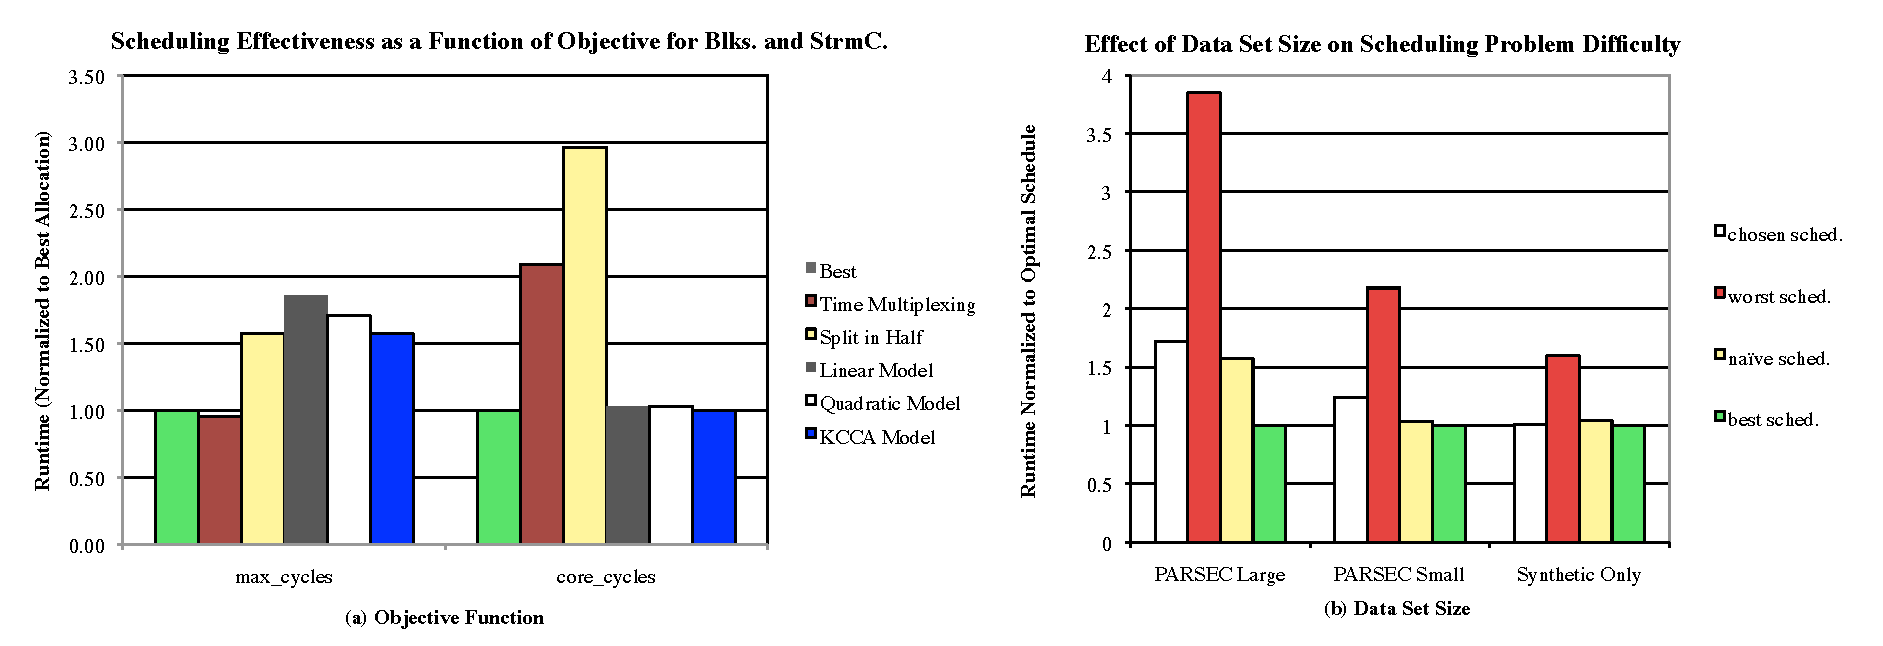
\includegraphics[width=1.0\textwidth]
        {Figures/case_study_outcome.pdf}}
        \caption{\label{fig:case_study_outcome}  (a) The performance
          of various scheduling methodologies and objective functions
          for one scheduling problem, normalized to the globally
          optimal schedule's performance.  The scheduler tries to
          minimize each objective function.  (b) The effect of
          benchmark size on the difficulty of the scheduling problem.
          The average chosen schedule performance, global worst case
          and naive scheduling case are normalized to the globally
          optimal schedule's performance for each dataset. The
          scheduling decision is Blackscholes vs. Streamcluster, the
          objective function is to minimize runtime.
 }
\end{figure*}

We found that predictive modeling has potential to successfully manage
some applications, depending on the scheduler's objective function.
For example, if the objective is to minimize energy, the approach
works quite well.  However, if the objective is to minimize the time
it takes to complete both applications, the naive baselines, such as
splitting the machine in half or time-multiplexing, often performed as
well or significantly better than model-based
allocation. Figure~\ref{fig:case_study_outcome}(a) presents an example
of these results. More importantly, our conclusions about the value of
model-based scheduling would have been different had we \emph{not}
simulated the entire execution of benchmarks, with large input sets,
for all possible allocations.

\begin{figure}[tb]
  \begin{center}
    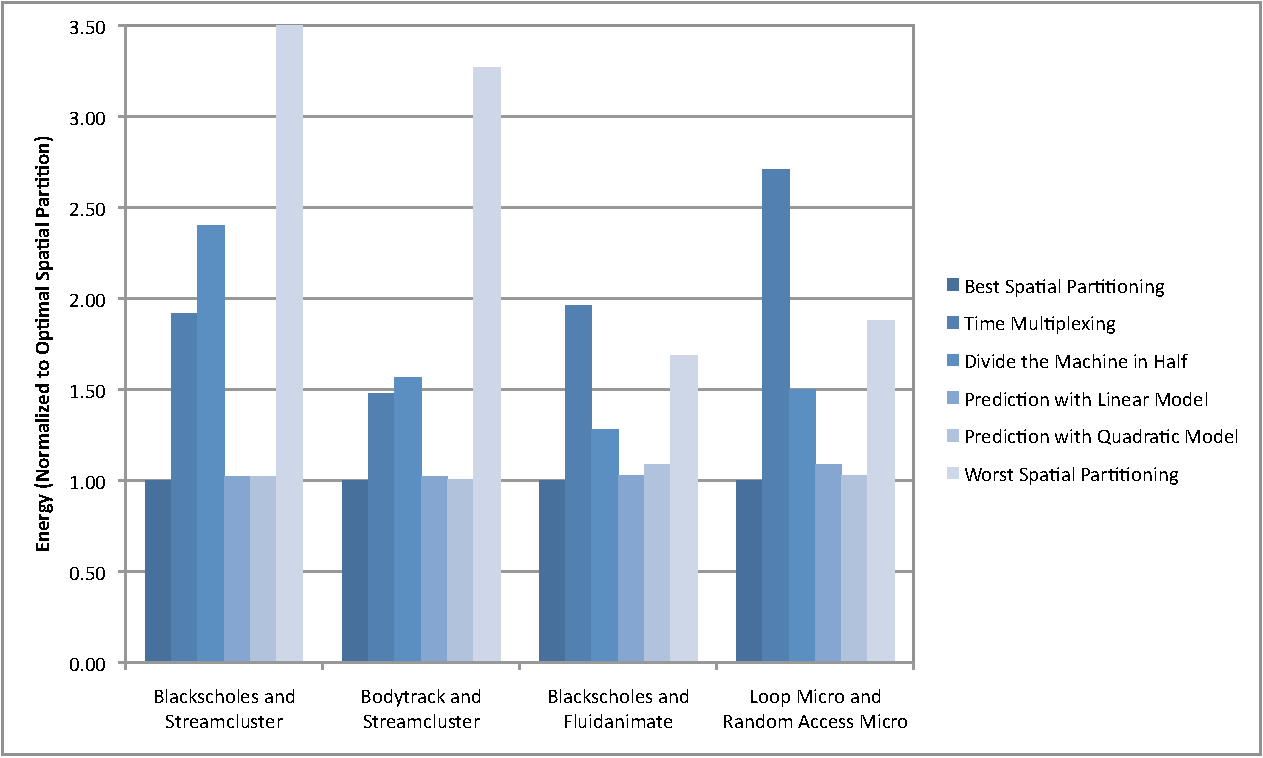
\includegraphics[width=\linewidth]{Figures/scheduling_results_energy.pdf}
  \end{center}
  \caption{Comparison of the effectiveness of different scheduling
    techniques normalized to our quadratic model-based approach.  The
    metric (sum of cycles on all cores + 10$\times$ sum of off-chip
    accesses) is a proxy for energy, so lower numbers are better.}
  \label{fig:scheduling_results}
\end{figure}




Figure~\ref{fig:scheduling_results} shows the results of our
scheduler's decisions based on the runtime performance data as
compared with several alternatives: the optimal allocation, naively
giving each application half of the machine, or time-multiplexing each
application across the entire machine.  

The time-multiplexing scheme
first runs the first application to completion and then runs the
second application to completion.  More fined-grained
time-multiplexing could lead to longer runtimes due to cache
interference effects and other context swap overheads.

We do no show results for the GPRS and KCCA as we found that they were extremely non-convex and as a result often produced very poor results when paired with our optimizer. The simple linear and quadratic models perform much better with only a small set of sample points and have significantly lower overhead.

The results
show that using runtime data to perform more intelligent scheduling
can lead to a significant savings in time and energy.  Our approach
beats naively dividing the machine by 65\% and time multiplexing by
100\% on average. Furthermore, it is within a few percent of optimal
every time.  The worst-case results show that the penalty for poor
decision making can be quite large, with an energy cost 3.25$\times$
greater than our allocation on average.

As the number of cores and other shared resources grows on chip, this
will increase the number of possible allocations, thereby widening the
performance gap between good and bad schedules.  Additionally, we
expect that much more code will be tuned for parallel execution, and
exhibit a greater variety of behaviors.  As a result, there will more
likely be disjoint resource requirements among applications available
to co-schedule.  We believe hardware measurement-based scheduling will
thus prove even more effective.


\subsection{\pacora Feasibility in a Real System}
Our static framework was designed to test the effectiveness of \pacora's model-based convex optimization for allocating resources.  We used it to experiment with the accuracy of different types of models and test the quality of the resource allocation decisions. Data is collected online by running application benchmarks on a recent x86 processor running Linux-2.6.36.  The measured data is processed using Python and then fed to MATLAB~\cite{matlab} to build the RTFs.  MATLAB uses the RTFs to make resource allocation decisions.  We compare performance of the chosen resource allocations with the actual measured performance of all possible resource allocations to test quality of the resource allocation decisions. We use CVX~\cite{cvx} in MATLAB to perform the convex optimization for building RTFs and making resource allocation decisions.  We chose this static approach because it let us test many applications, 44 in total, and many resource allocations rapidly.

\subsubsection{Platform}

To collect data, we use a prototype version of Intel's Sandy Bridge x86 processor that is similar to the
commercially available client chip, but with additional hardware
support for way-based LLC partitioning.
The Sandy Bridge client chip has 4 quad-issue out-of-order
superscalar cores, each of which supports 2 hyperthreads using
simultaneous multithreading~\cite{IntelRefManual:2011}.
%Each core has private \wunits{32}{KB} instruction and data caches, as well as a
%\wunits{256}{KB} private non-inclusive L2 cache.
The LLC is a 12-way
set-associative \wunits{6}{MB} inclusive L3 cache, shared among all
cores using a ring-based interconnect.
%All three cache levels are write-back.
The cache partitioning mechanism is way-based and works by modifying the
cache-replacement algorithm.  To allocate cache ways, we assign a subset of
the 12 ways to a set of hyperthreads, thereby allowing only those hyperthreads to replace data in those ways.

%Way allocations can be completely private,
%completely shared, or overlapping.  Although all cores can hit on data stored in
%any way, a core can only replace data in its assigned
%ways.   Data is not flushed when the way allocation changes.

We use a customized BIOS that enables the cache partitioning
mechanism, and run unmodified Linux-2.6.36 for all of our experiments.
To allocate cores, we use the Linux \texttt{taskset} command to pin applications to
sets of hyperthreads. The standard Linux scheduler performs the scheduling for applications within these containers of hyperthreads. For our experiments we consider each hyperthread to be an independent core. To minimize inter-application interference, we first assign both hyperthreads available in one core before moving on to the next core. For example, a 4-core allocation from \pacora represents 4 hyperthreads on 2 cores on the machine.

\subsubsection{Performance and Energy Measurement}

To measure application performance, we use the \texttt{libpfm}
library~\cite{Eranian:OLS06,Perfmon2}, built on top of the
\texttt{perf\_events} infrastructure in Linux, to
access available performance counters~\cite{Intel:Manual2012}.

To measure on-chip energy, we use the energy counters available on
Sandy Bridge to measure the consumption of  the entire socket and also
the total combined energy of cores, their private caches, and the
LLC. We access these counters using the Running Average Power Limit
(RAPL) interfaces~\cite{Intel:Manual2012}.  %The counters measure power
%at a $1/2^{16}$ second granularity.

%In addition, we use a FitPC external multimeter to measure at the wall socket the power
%consumed by the entire system, at a
%\wunits{1}{second} granularity.
%We correlate the wall power data with the data collected from the hardware energy counters
%using time stamps.  We observed less than one second of delay in these
%measurements consistently across all experiments.  Together, these
%mechanisms allow us to collect accurate energy readings over the
%entire course of an application's execution.

\subsubsection{Description of Workloads}

Our workload contains a range of applications from three different
popular benchmark suites: SPEC CPU 2006~\cite{SPEC2006},
DaCapo~\cite{dacapo}, and PARSEC~\cite{parsec}. We selected this set of applications to represent a wide variety of possible resource behaviors in order to properly stress \pacora's RTFs. We include some additional applications to broaden the
scope of the study, and some microbenchmarks to exercise certain
system features.

The \textbf{SPEC CPU2006} benchmark suite~\cite{SPEC2006} is a
CPU-intensive, single-threaded benchmark suite, designed to stress a
system's processor, memory subsystem, and compiler.  Using the
similarity analysis performed by Phansalkar \emph{et
al.}~\cite{Phansalkar:ISCA2007}, we subset the suite, selecting 4
integer benchmarks (\texttt{ astar}, \texttt{ libquantum}, \texttt{ mcf}, \texttt{ omnetpp}) and 4
floating-point benchmarks (cactusADM, calculix, lbm, povray).  Based
on the characterization study by Jaleel~\cite{Jaleel:TR2007}, we also
pick 4 extra floating-point benchmarks that stress the LLC: \texttt{ GemsFDTD},
\texttt{ leslie3d}, \texttt{ soplex} and \texttt{ sphinx3}.  When multiple input sets are
available, we pick the single \textit{ref} input indicated by~\cite{Phansalkar:ISCA2007}.

We include the \textbf{DaCapo} Java benchmark suite as a
representative of managed-language workloads. We use the latest 2009 release, which consists of a set of open-source, real-world
applications with non-trivial memory loads, and includes both client and
server-side applications.

The \textbf{PARSEC} benchmark suite is intended to be representative
of parallel real-world applications~\cite{parsec}. PARSEC
programs use various parallelization approaches, including data- and
task-parallelization. We use native input sets and the \texttt{ pthreads} version for all benchmarks, with the exception of
\texttt{freqmine}, which is only available in OpenMP.

We add four \textbf{additional parallel applications} to help ensure
we cover the space of interest: \texttt{ Browser\_animation} is a
multithreaded kernel representing a browser layout animation; \texttt{
  G500\_csr} code is a breadth-first search algorithm; \texttt{ Paradecoder} is a parallel
speech-recognition application that takes audio waveforms of human
speech and infers the most likely word sequence intended by the
speaker; \texttt{ Stencilprobe} simulates heat transfer in a fluid
using a parallel stencil kernel over a regular
grid~\cite{Kamil:Stencilprobe}.

We also add two \textbf{microbenchmarks} that stress the memory
system and cause increased interference between applications: \texttt{ stream\_uncached} is a memory and on-chip bandwidth hog
that continuously brings data from memory without caching it, while
\texttt{ ccbench} explores arrays of different sizes to determine the
structure of the cache hierarchy.

Using a performance characterization of the applications, we select a subset of the benchmarks that are representative of different possible responses to resource allocations in order to reduce our study to a feasible size.  Similar to \cite{Phansalkar:ISCA2007}, we use machine learning to select representative benchmarks.  We use a
hierarchical clustering algorithm~\cite{Phansalkar:ISCA2007} provided by the Python library \texttt{scipy-cluster} with the \textit{single-linkage} method.  The feature vector contains parameters to represent core scaling, cache scaling, prefetcher sensitivity and bandwidth sensitivity.  The clustering algorithm uses Euclidean distance between vectors to determine clusters.

The clustering results in 6 clusters representing the following (applications at the cluster center are listed in parenthesis):
 \begin{itemize}\itemsep0pt \parskip0pt \parsep5pt
\item no scalability, high cache utility, (\texttt{ 429.mcf})
\item no scalability, low cache utility, (\texttt{ 459.gems\-FDTD})
\item high scalability, low cache utility, (\texttt{ ferret})
\item limited scalability, high cache utility, (\texttt{ fop})
\item limited scalability, low cache utility, (\texttt{ dedup})
\item limited scalability, low bandwidth sensitivity, (\texttt{ batik})
\end{itemize}

%First, we create a feature vector for each application using the values in the previous subsection:
%1) execution time as we increase the number of threads; 2) execution time as we increase the LLC size; 3) prefetcher sensitivity; and 4) bandwidth sensitivity. All metrics are normalized to the interval $[0,1]$. In total we use vectors with 19 features ($7+10+1+1$).

%The clustering algorithm finds the smallest Euclidean distance of a pair of feature vectors and forms a cluster containing that pair. It continues selecting the next smallest distance between a pair and forms another cluster. Linkage criteria can be used to adjust cluster formation. The single-linkage we selected uses the minimum distance between a pair of objects in different clusters to determine the distance between them.

\subsubsection{RTF Experiments}
\begin{figure*}[!t]
	\begin{center}	
		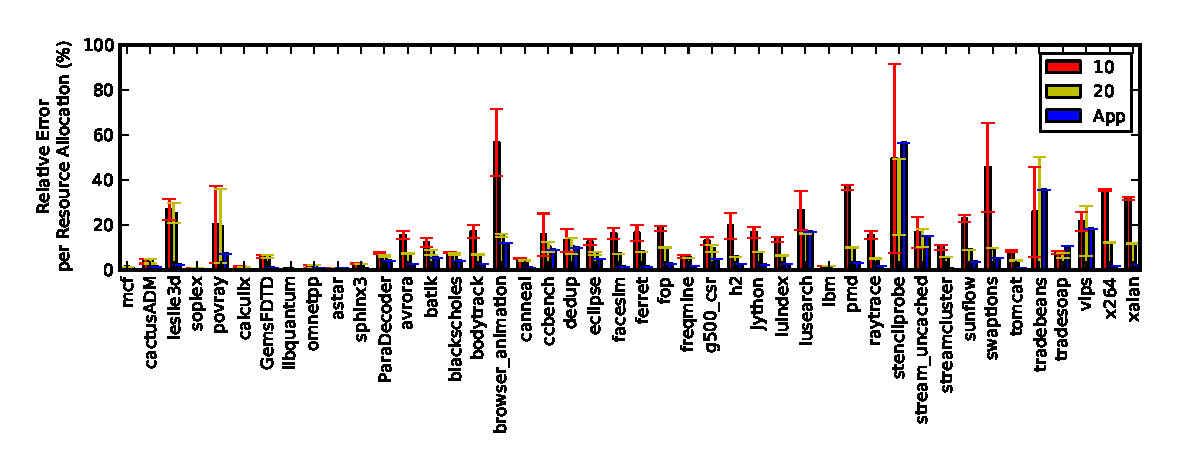
\includegraphics[bb=0 0 576 216,width=\textwidth]{Figures/model_accuracy.pdf}
		\caption{1-norm of relative error from RTF predicted response time compared to actual response time.  The actual response time is the median over 3 trials. 10 and 20 represent RTFs built with 10 and 20 training points respectively.  App represents the variability (average standard deviation) in performance of the application between the 3 trials.}
		\label{model_accuracy}
	\end{center}
\end{figure*}
To test the effectiveness of our RTFs in capturing real application behavior, we measure each of our 44 benchmarks running alone on the machine for all possible resource allocations of cache ways and cores.  Cores can be allocated from 1--8 and cache ways from 1--12 resulting in 96 possible allocations for each application.   We use a genetic algorithm design of experiments~\cite{bates-aes03} to select 10 and 20 of the collected allocations to build the RTFs.  We also experimented with building RTFs with more data points but found that they provided little improvement over 20~\cite{pacora_tr}.  We then use the model to predict the performance of every resource allocation and compare it with the actual measured performance (median value of 3 trials) of that resource allocation.  We built 3 different models from 3 trials and tested each of them against median measured value.

Figure~\ref{model_accuracy} shows the 1-norm of the relative error of the predicted response times per resource allocation for an RTF built with 10 training points and one built with 20.  The average error per point is 16\% for an RTF built with 10 training points and 9\% for an RTF built with 20 training points.  We also calculated the percentage variability (average standard deviation) for each resource allocation in the application between the 3 trials (shown as ``App'' in Figure~\ref{model_accuracy}).  The average variability is 9\%, so we can see that \pacora's RTFs are not much more inaccurate than the natural variation in response time in the application.  It is not for possible an RTF to be more accurate than the application variability, and we can also see that applications with higher variability result in RTFs with larger relative errors, (\emph{e.g.,} \texttt{stencilprobe}, \texttt{ tradebeans}).  Section~\ref{discuss} discusses application variability in more detail.

\subsubsection{Resource Allocation Experiments}
\begin{figure}[!t]
	\begin{center}	
		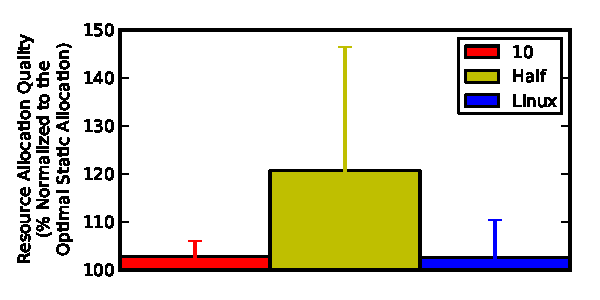
\includegraphics[bb=0 0 288 144,width=\columnwidth]{Figures/decision_quality.pdf}
		\caption{Resource allocation decisions for each pair of the cluster representative applications compared equally dividing the machine and a shared resources Linux baseline. Quality is measured is allocation performance divided by performance of the best possible allocation.}
		\label{decision_quality}
	\end{center}
\end{figure}


Using the RTFs built for the applications, we let \pacora make static resource allocations for all possible pairs of the cluster representative applications.  We then run an exhaustive study of all possible resource allocations for each pair on our Sandy Bridge-Linux platform, measure the performance, and compare it with the best performing, \emph{i.e.,} optimal, resource allocation.  We also compare this result to equally dividing the resources between the two applications and to sharing all of the resources using the standard Linux scheduler.

%how \pacora's decisions compared with the optimal allocation, equally dividing the machine, and the Linux baseline for each pair of the cluster representative applications.
Figure~\ref{decision_quality} shows these results for our 10 point RTFs. As we might expect, simple naive heuristics do not perform well, and dividing the machine in half is around 20\% slower than either \pacora or standard Linux.
 \pacora's resource allocations are 2\% from the optimal static allocation on average.  Using shared resources with the standard Linux scheduler performs similarly but with a higher standard deviation.  The shared resources comparison is interesting: while most of the time sharing resources can result in higher utilization, as the applications can dynamically take advantage of available resources, in some cases the interference between applications was so harmful to performance that on average optimal static partitioning performs slightly better.  As a result \pacora is able to provide performance comparable to Linux scheduling on shared resources with more predictable performance on average (lower worst cases).  Additionally, as the shown in the next Section, \pacora's resource allocation decisions do not need to be static, but can be made dynamically to adjust to the changing needs of the applications.
%These results indicate the \pacora is able to get a near optimal resource allocation and match the performance of the traditional Linux scheduler with more predictability.

\subsubsection{Effect of Model Accuracy on Decision Quality}

\begin{figure}[!t]
	\begin{center}	
%		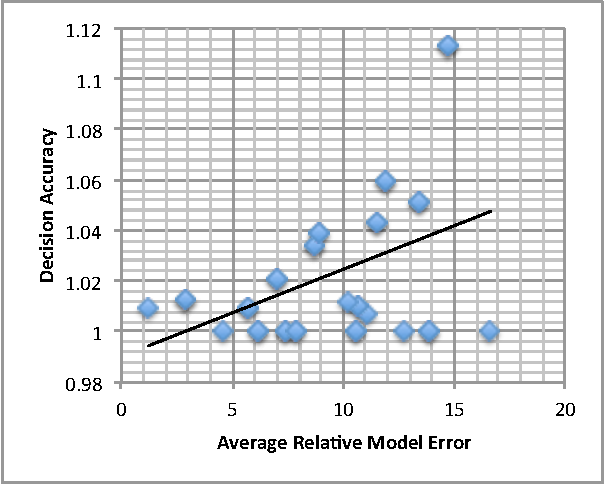
\includegraphics[width=0.9\textwidth]{cluster_decision_accuracy.pdf}
		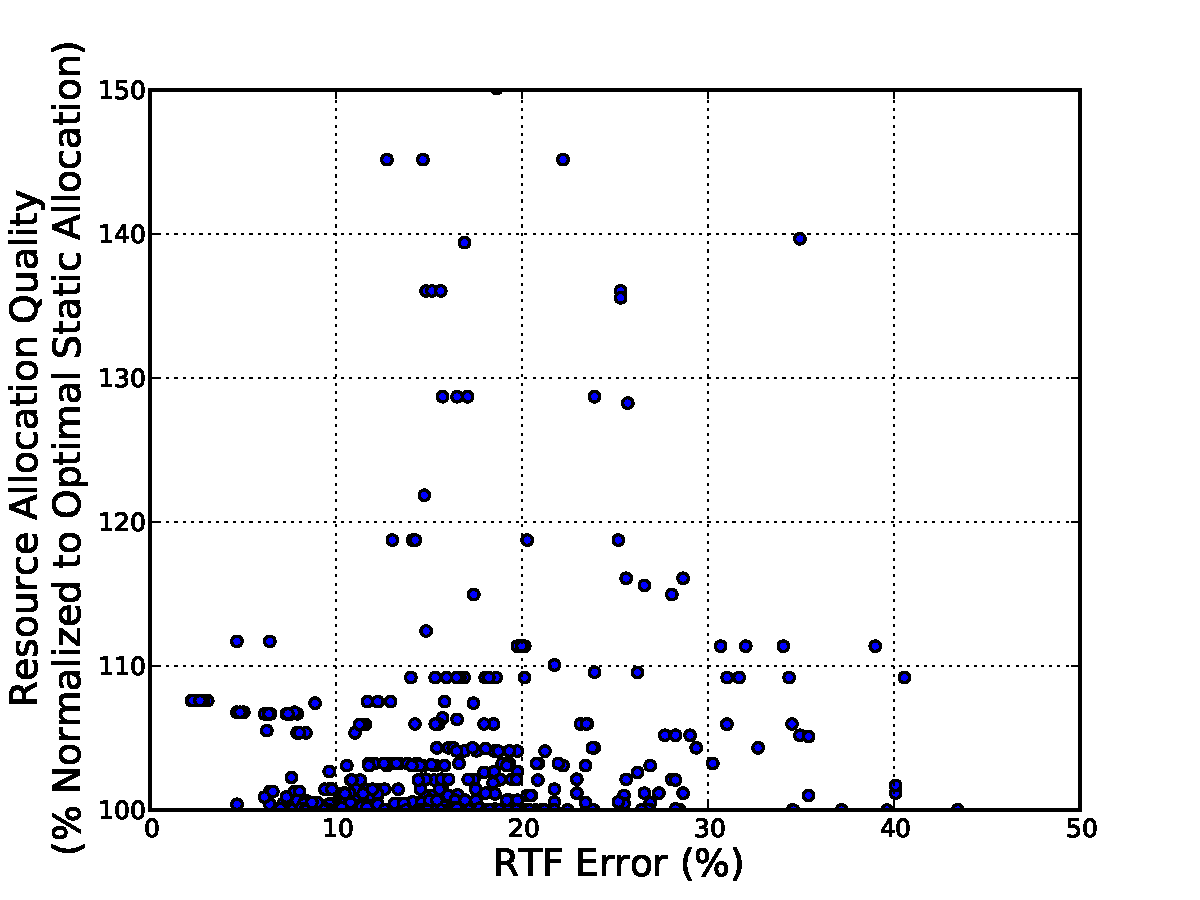
\includegraphics[bb=0 0 576 432,width=\columnwidth]{Figures/accuracy_quality.pdf}
		\caption{Effect of Model Accuracy on Decision Quality. The x axis represents the combined relative error of all RTFs used in the decision.}
		\label{accuracy_quality}
	\end{center}
\end{figure}


There are two main sources of challenges for \pacora's design: performance non-convexity and performance variability. 
The main concern with performance non-convexity and variability is their effects on the accuracy of the response time functions.  However, an important result we have found while evaluating \pacora is that model accuracy has less impact on the quality of resource allocation decisions than we anticipated.  When experimenting with possible models for the RTFs, we found that while some models were always a little too inaccurate and did degrade the performance of the resource allocation decisions, once a model crossed a certain threshold of accuracy then better models provided insignificant improvement in resource allocation decisions. Figure~\ref{accuracy_quality} shows the effect of model accuracy on the quality of the resource allocation decisions made using the RTF model in Equation~\ref{rtf_eq}.  Although there is a slight correlation between model accuracy and decision quality, many decisions with inaccurate models still result in near optimal allocations.  This effect enables \pacora's model-based design to be feasible in a noisy system with real applications.

